Durant notre première séance de laboratoire pour le cours de physique des télécommunications, nous avons dimensionné une antenne patch alimentée par une ligne microstrip à l'aide du logiciel FEKO. Pour cela nous avons procédé par étapes, partant d'un design simple et parfaitement symétrique auquel nous avons petit à petit ajouté ou modifié des éléments pour arriver à la version finale remplissant toutes les spécifications.

A la fin de la séance, nous avons obtenu une antenne dont les caractéristiques simulés étaient un coefficient de réflexion minimal de \SI{-27.43}{\deci\bel} à la fréquence de \SI{2.398}{\giga\hertz}\footnote{le cahier des charges nous imposait un coefficient de réflexion de \SI{-6}{\deci\bel} à la fréquence d'utilisation de l'antenne, c'est-à-dire \SI{2.4}{\giga\hertz}}, et un gain maximal de \num{2.54}.

Cette antenne sera ensuite testée expérimentalement lors de la troisième séance. Dans ce chapitre, nous allons détailler les différentes étapes qui nous ont amené au dimensionnement final de notre antenne.

\subsection{Antenne sur un diélectrique infini}
Pour commencer, nous avons simplement simulé un patch rectangulaire en matériau conducteur parfait posé sur un matériau diélectrique de même permittivité électrique que le PCB utilisé en pratique pour fabriquer notre antenne, mais considéré dans un premier temps sans pertes. Pour ce qui est des dimensions (longueur et largeur) du patch, nous avons utilisé les formules qui nous étaient fournies. La figure \ref{fig:rayonnement_11} nous donne la directivité ainsi que le gain de l'antenne pour des valeurs de $\phi$ de \SI{0}{\degree} et \SI{90}{\degree}.
\begin{figure}[htbp]
  \centering
  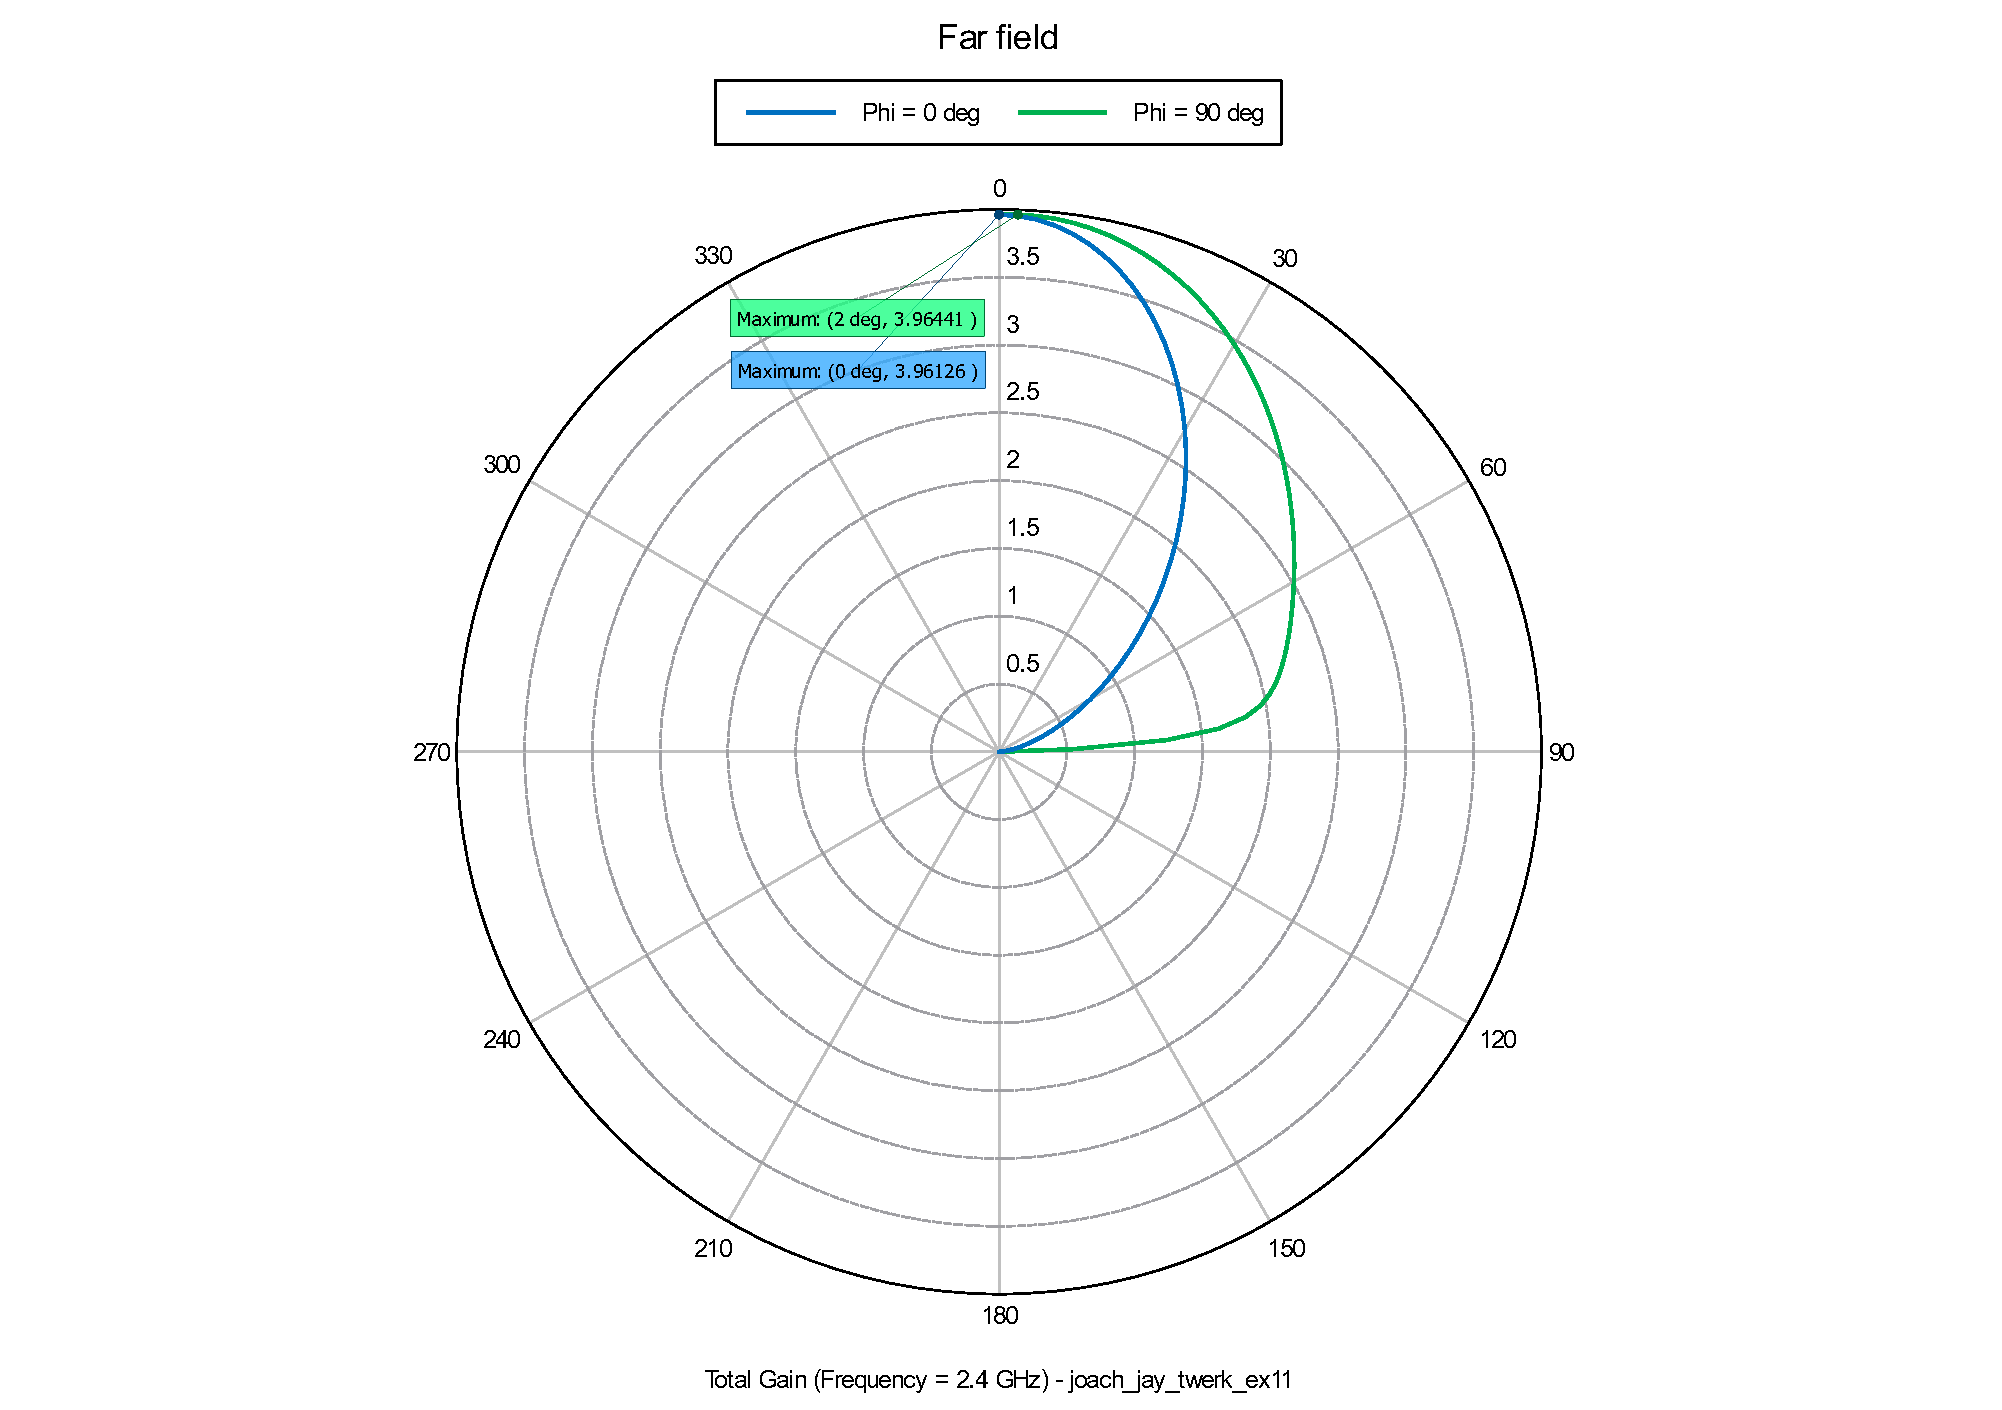
\includegraphics[width=\textwidth]{rayonnement11_annotation.pdf}
  \caption{Diagramme de rayonnement du gain [généré avec PostFeko]\label{fig:rayonnement_11}}
\end{figure}
Pour les deux valeurs de $\phi$, la directivité maximale est de \SI{0}{\degree}.

Nous nous sommes aussi intéressés au coefficient de réflexion de l'antenne ainsi qu'à sa fréquence de résonance.
\begin{figure}[htbp]
  \centering
  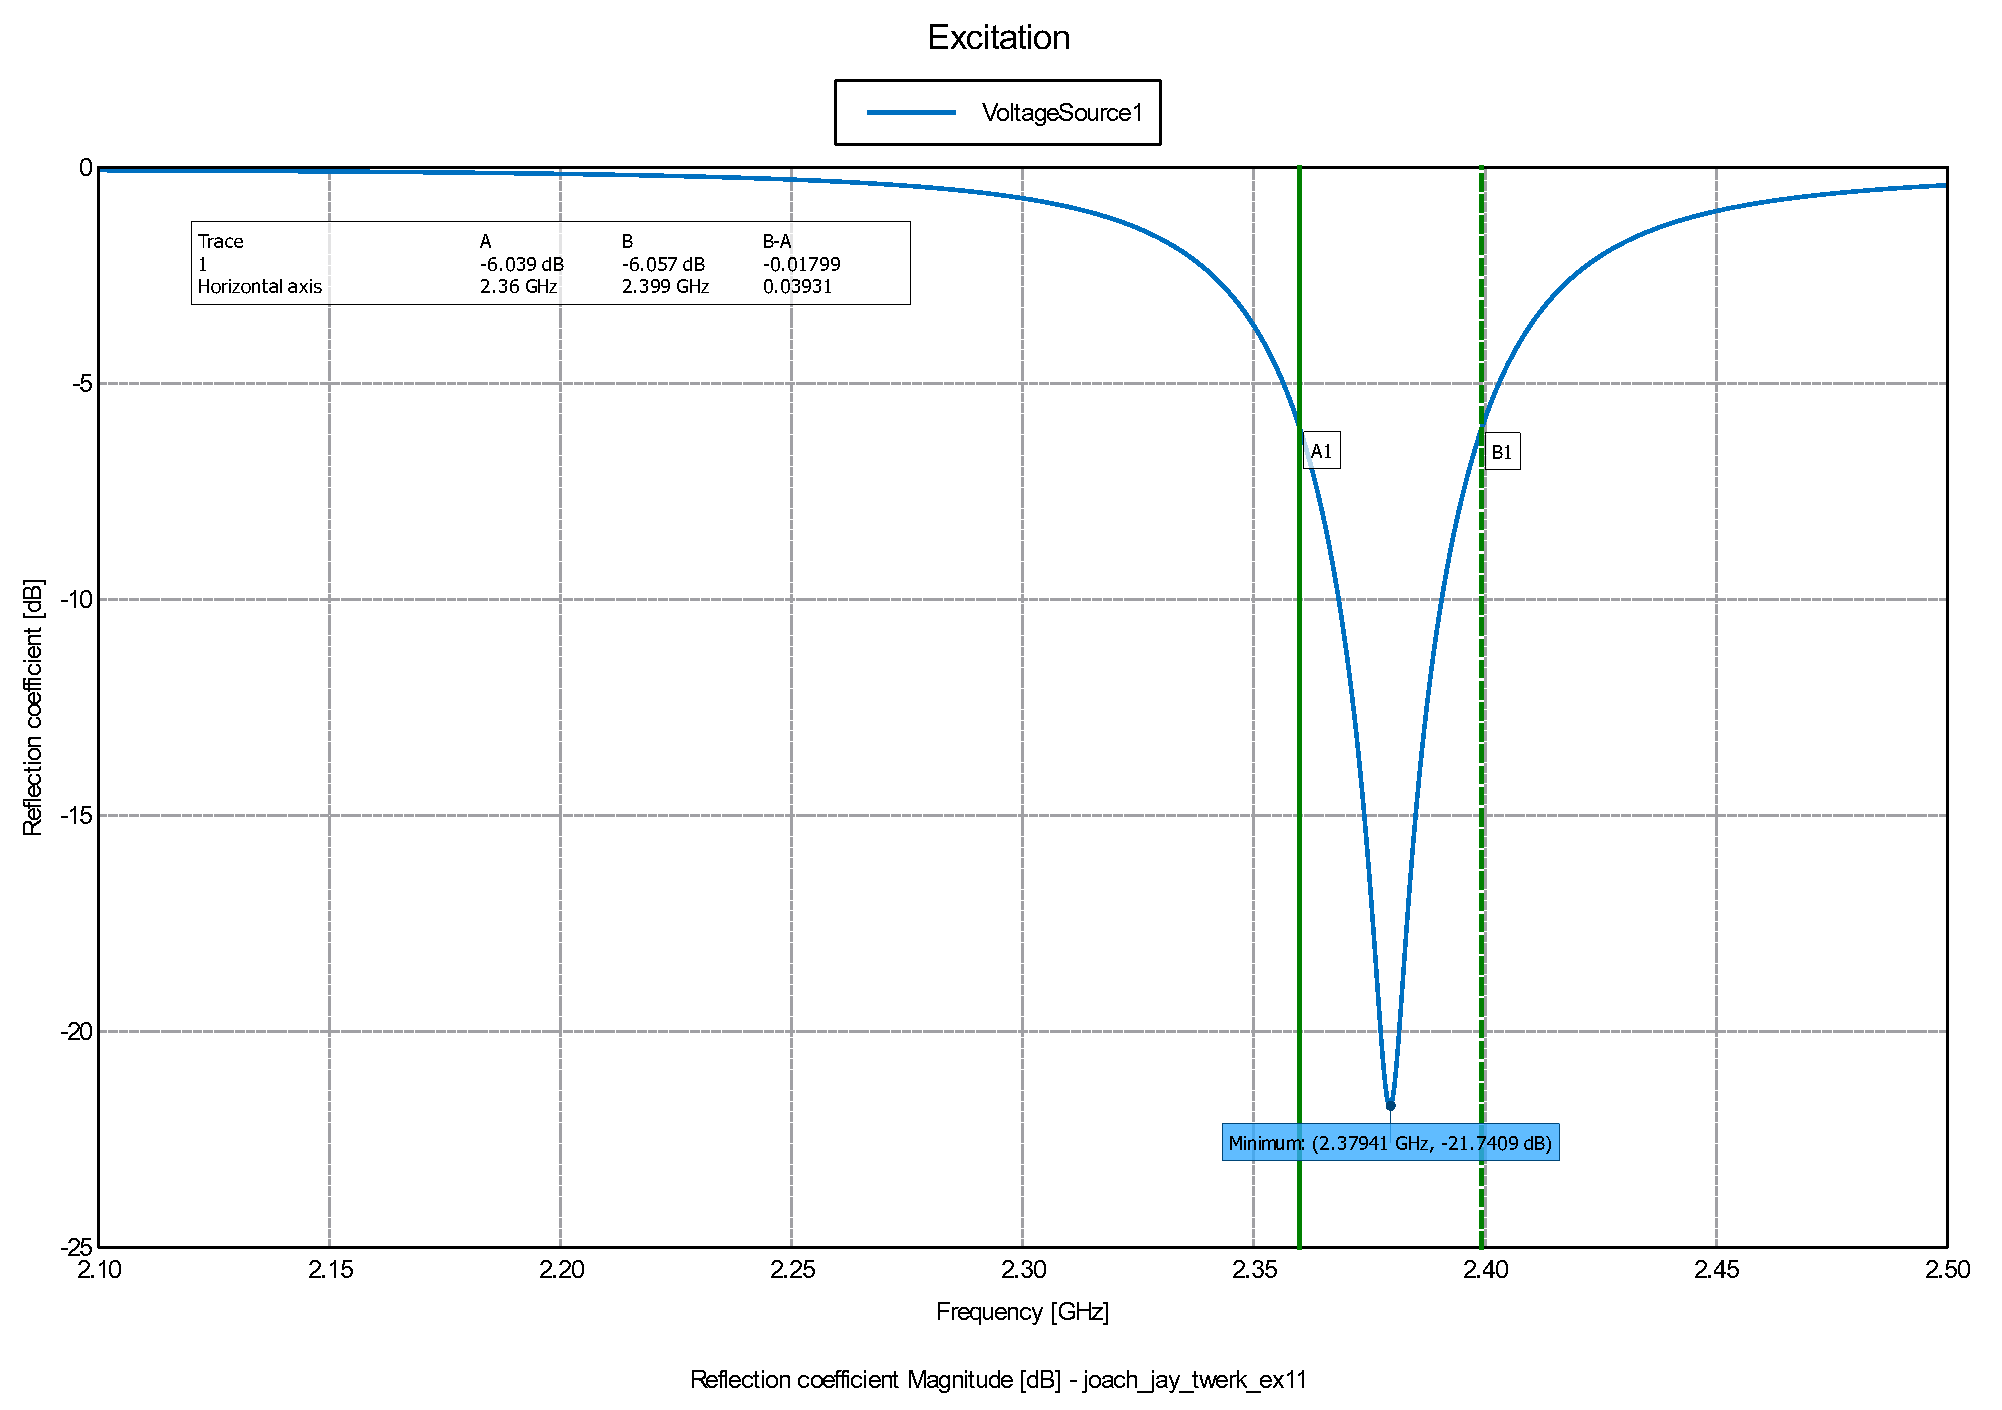
\includegraphics[width=\textwidth]{reflection11_annotation.pdf}
  \caption{Coefficient de réflexion en fonction de la fréquence [généré avec PostFeko]\label{fig:reflection11_}}
\end{figure}
La figure \ref{fig:reflection11_} nous montre que la résonance de l'antenne se situe à \SI{2.38}{\giga\hertz} et qu'à cette fréquence le coefficient de réflexion vaut \SI{-21.8}{\deci\bel}. A la fréquence d'intérêt de \SI{2.4}{\giga\hertz}, ce coefficient vaut \SI{-6}{\deci\bel}. Il est aussi intéressant de noter la largeur de la bande passante\footnote{Définie ici comme l'intervalle de fréquence ou $\Gamma_L < \SI{-6}{\deci\bel}$} qui vaut dans ce cas près de \SI{0.04}{\giga\hertz}.

A partir de ces mesures, nous pouvons calculer le pourcentage de puissance délivrée à l'antenne à la fois à la fréquence de résonance et à \SI{2.4}{\giga\hertz}. Ce pourcentage est obtenu par la relation \ref{eqn:puissance délivrée}, qui nous donne une valeur de \SI{99.3}{\percent} à la fréquence de résonance et \SI{75.2}{\percent} à \SI{2.4}{\giga\hertz}.
\begin{equation}
\frac{P_L}{P_{in}} = 1-{\Gamma_L}^2
\label{eqn:puissance délivrée}
\end{equation}

%Note pour jojol: coeff de réflection c'est gamma majuscule, aka \Gamma_L (L pour load).
%Merci d'utiliser \SI! c'est vachement cool!
%Je me suis planté, la proportion absorbée c'est 1-(gamma)². Je m'occupe (ou me suis occupé) de corriger dans ce qui est déjà fait.
%Largeur des figures = \textwidth? Sinon je trouve qu'elles ne sont pas super lisibles
%NOTE POUR TWERKYTWERK : pour la largeur des figures je me suis 100pourcent inspiré des labos de thermo, je te laisse modifier la mise en forme à ta guise, je touche pas grand chose à ça

\subsection{Antenne sur un diélectrique fini}
Le pas suivante vers une antenne patch réelle consiste à remplacer le substrat infini par un carré de coté \SI{50}{\milli\meter}, c'est-à-dire la dimension du PCB de notre antenne. Ci-dessous, nous détaillons les changements dû à cette modification sur les différents paramètres déjà étudiés plus haut.

Premièrement, comme nous pouvons le voir sur la figure \ref{fig:reflection12_annotation},
\begin{figure}[htbp]
\centering
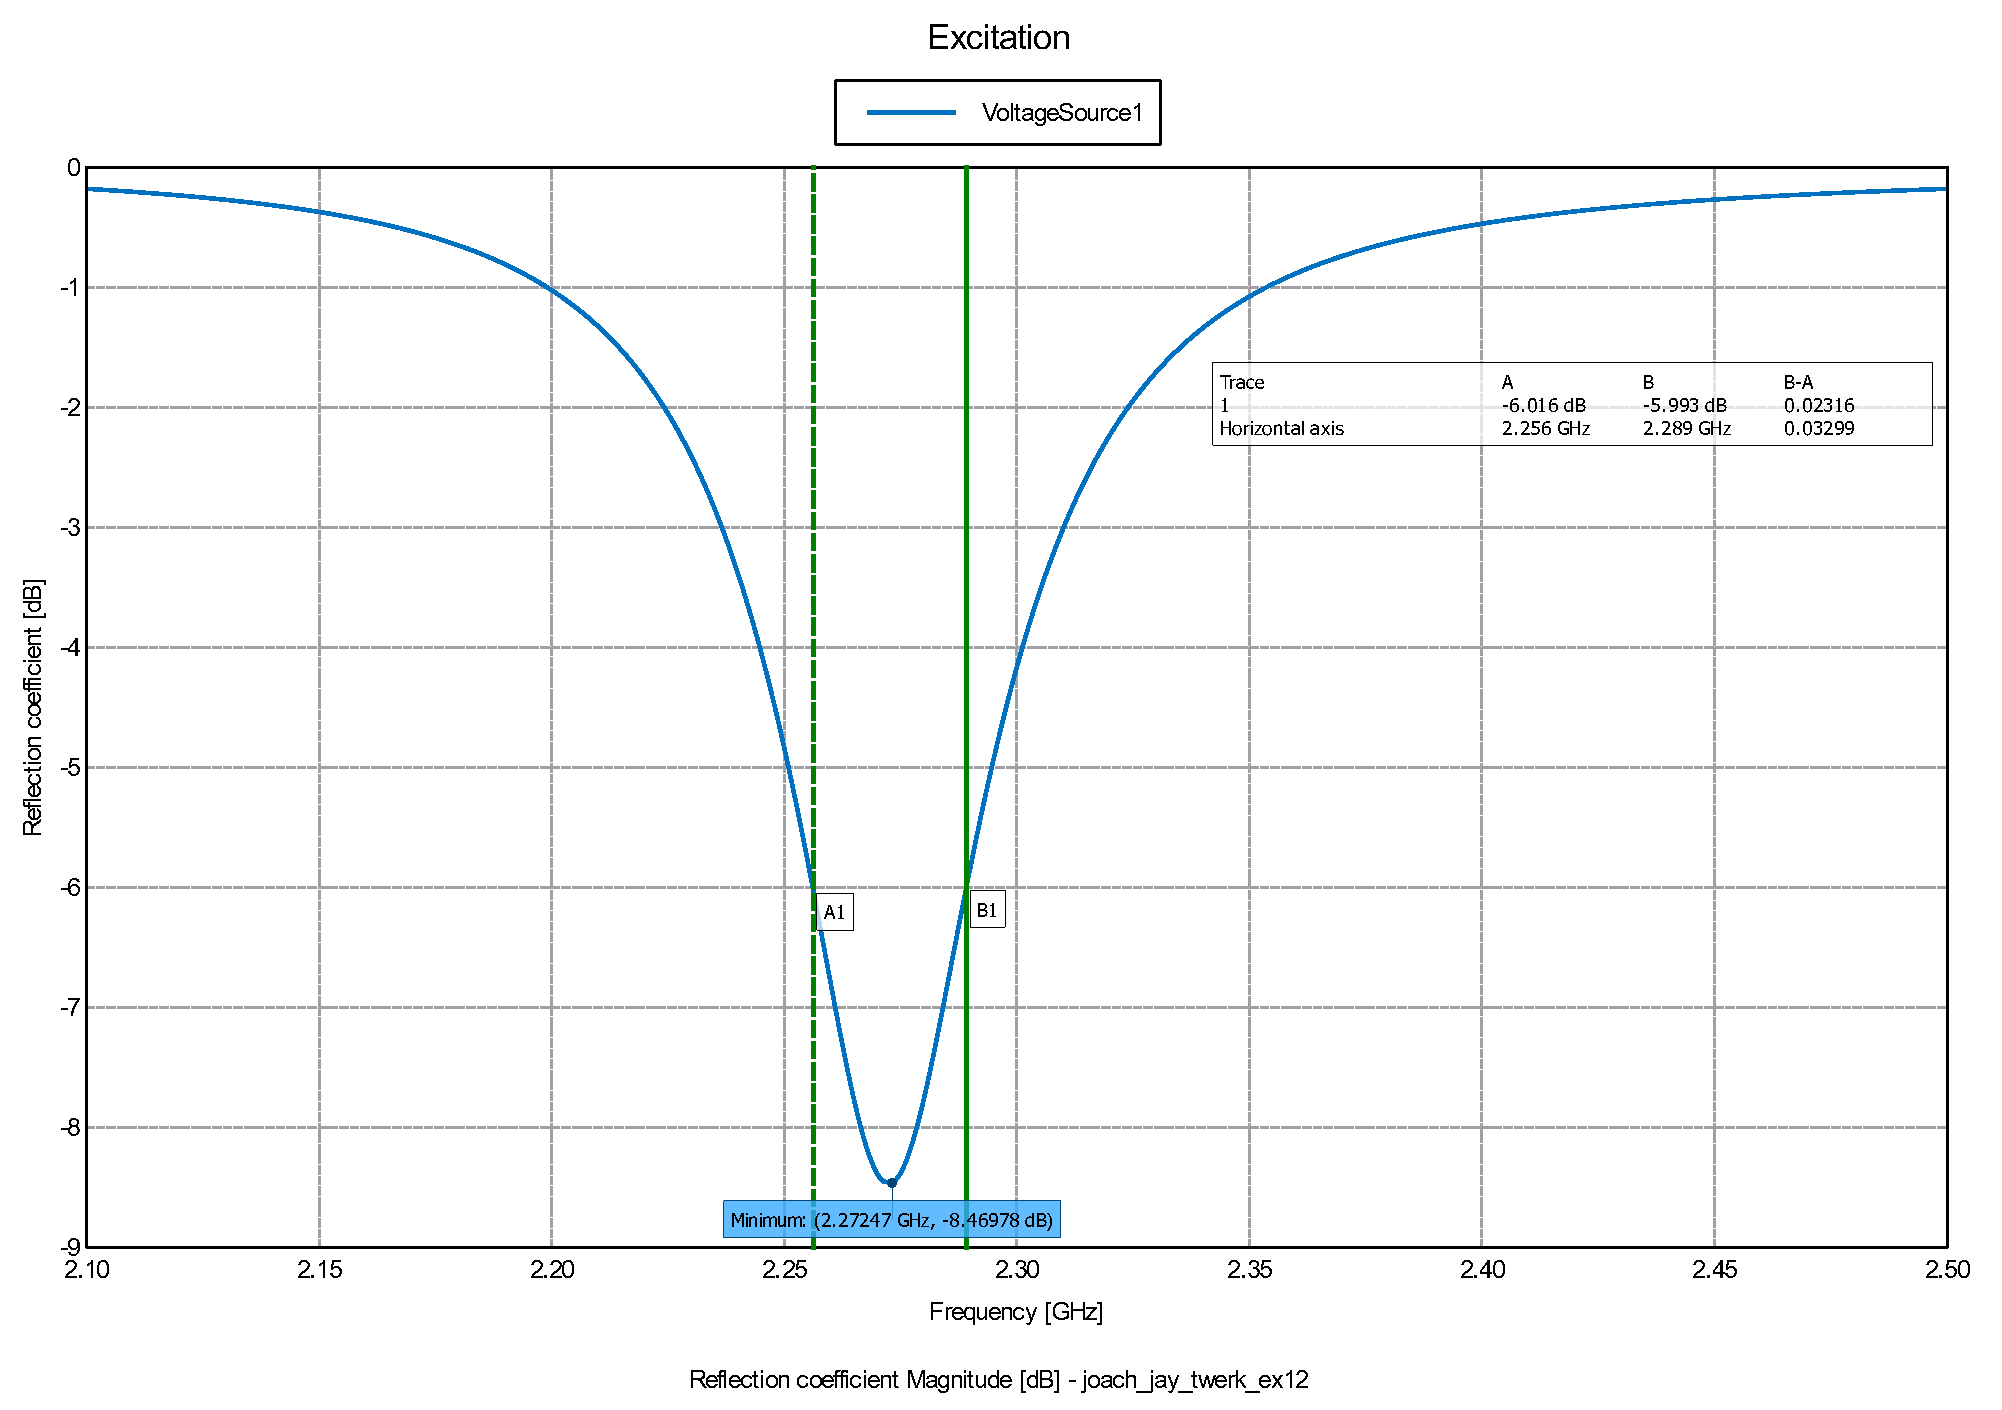
\includegraphics[width=\textwidth]{reflection12_annotation.pdf}
\caption{Coefficient de réflexion en fonction de la fréquence\label{fig:reflection12_annotation}}
\end{figure}
la fréquence de résonance s'est déplacée à \SI{2.27}{\giga\hertz} mais le coefficient de réflexion à surtout fortement augmenté pour prendre la valeur de \SI{-8.47}{\deci\bel}. La bande passante s'est elle aussi dégradée et ne vaut plus que \SI{0.033}{\giga\hertz}.

A nouveau, il est intéressant d'étudier le diagramme de rayonnement du gain de l'antenne, donné à la figure \ref{fig:rayonnement12_annotation}, où l'on remarque que la directivité maximale est à  \SI{0}{\degree} et le gain maximal à \SI{3.64} que ce soit pour $\phi = \SI{0}{\degree} ou  \SI{90}{\degree}$.
\begin{figure}
\centering
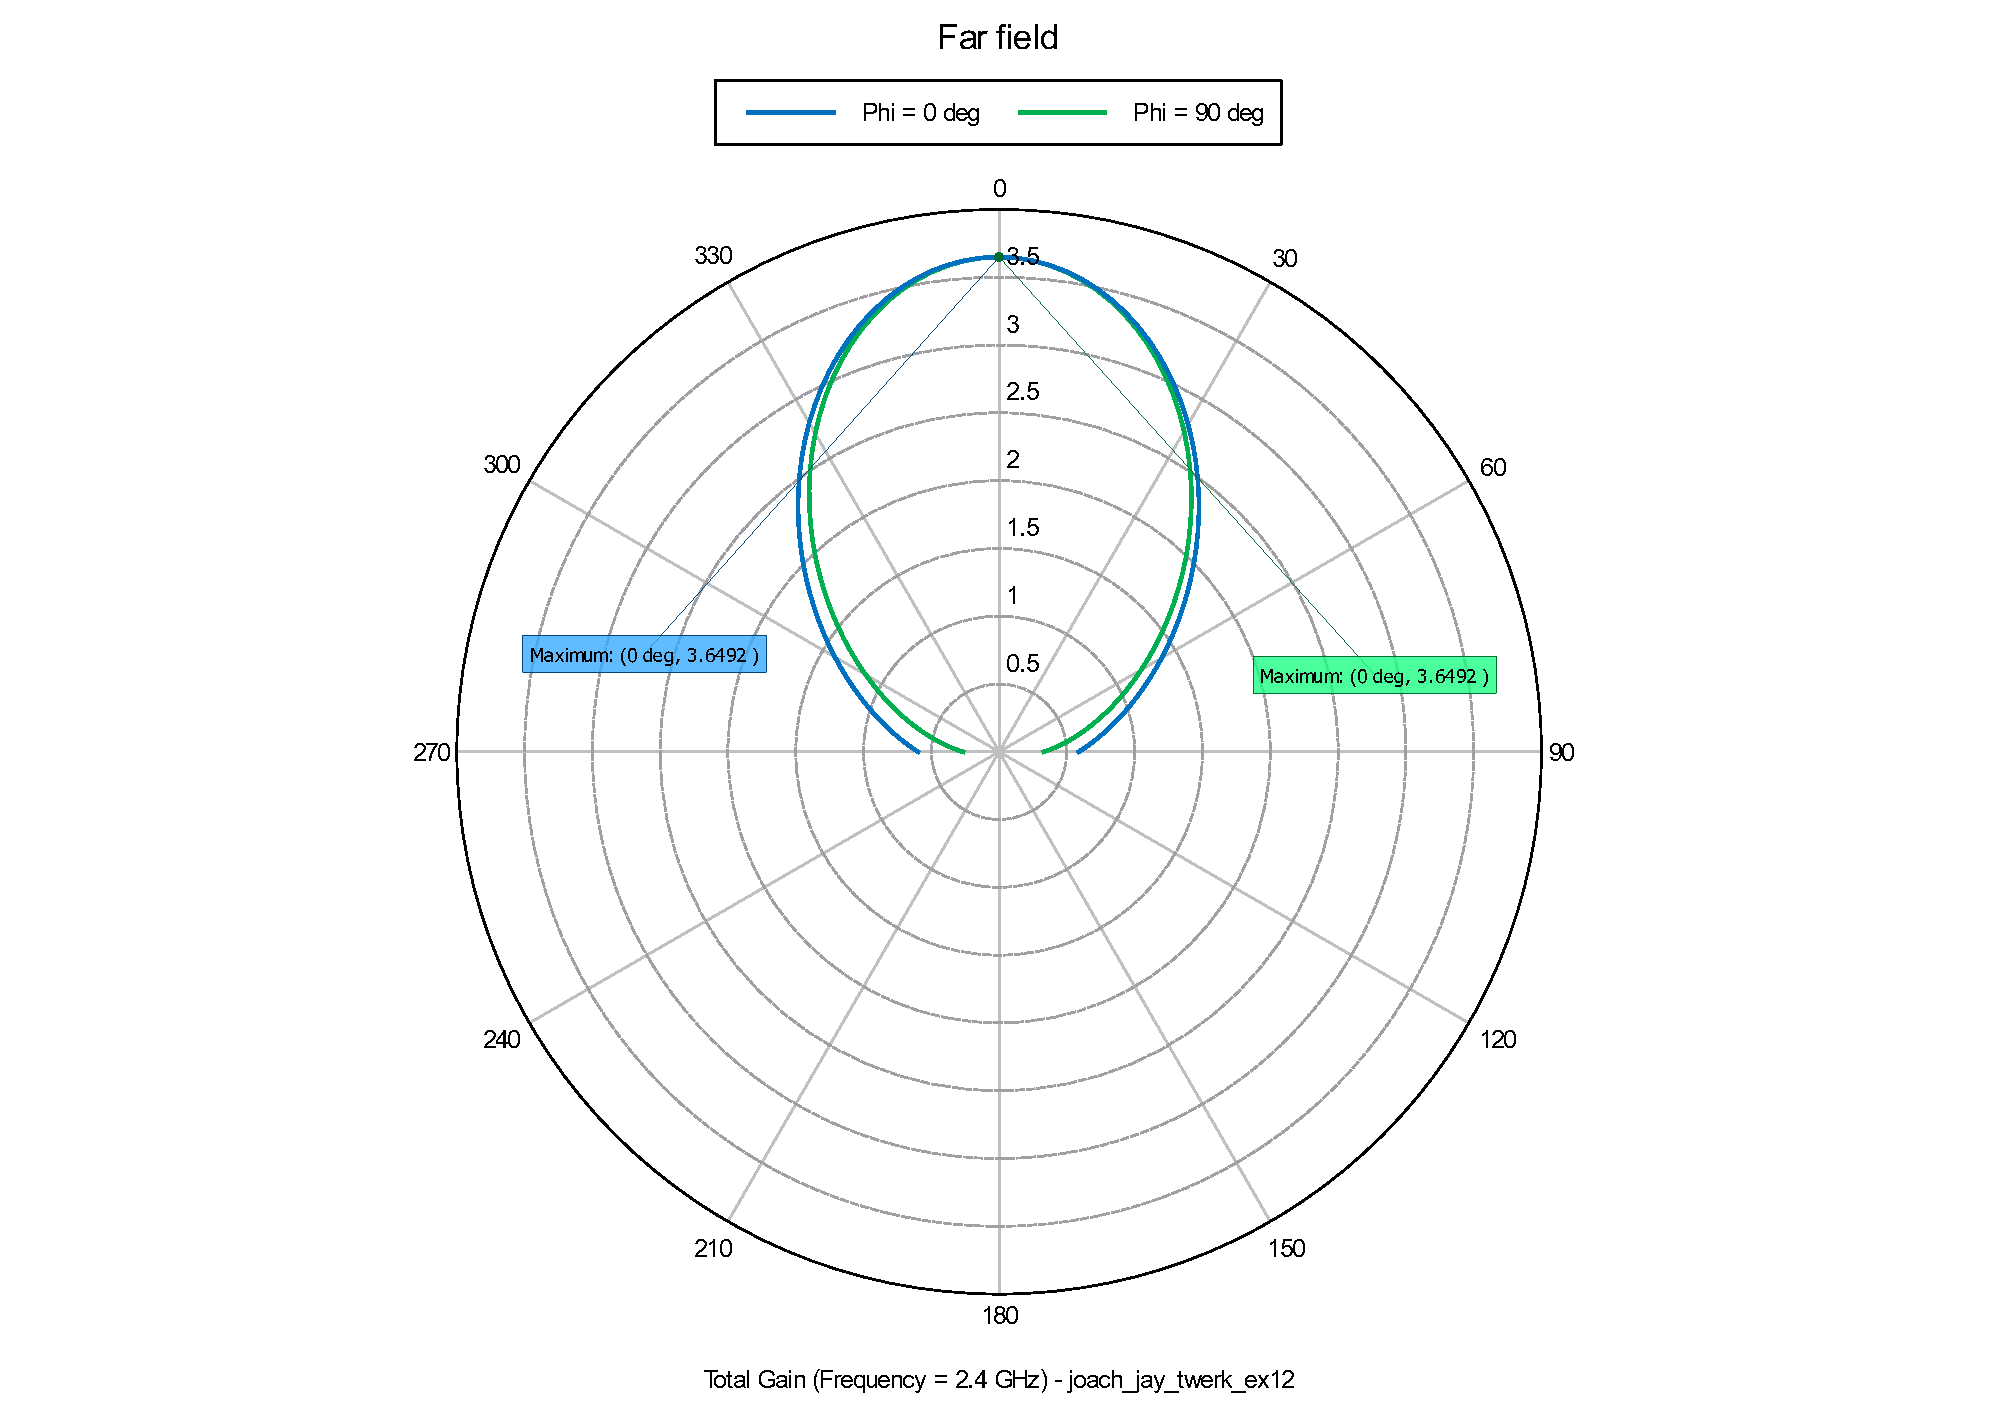
\includegraphics[width=\textwidth]{rayonnement12_annotation}
\caption{Diagramme de rayonnement de l'antenne sur diélectrique fini}
\label{fig:rayonnement12_annotation}
\end{figure}
Pour terminer, nous avons modifié le déphasage de sorte que $\tan{\delta} = 0.01$. Le gain diminue alors à \SI{2.64} et le coefficient de réflexion vaut \SI{-6}{\deci\bel} à la résonance, qui reste inchangée. (\ref{fig:reflection122_annotation}).
\begin{figure}[htbp]
\centering
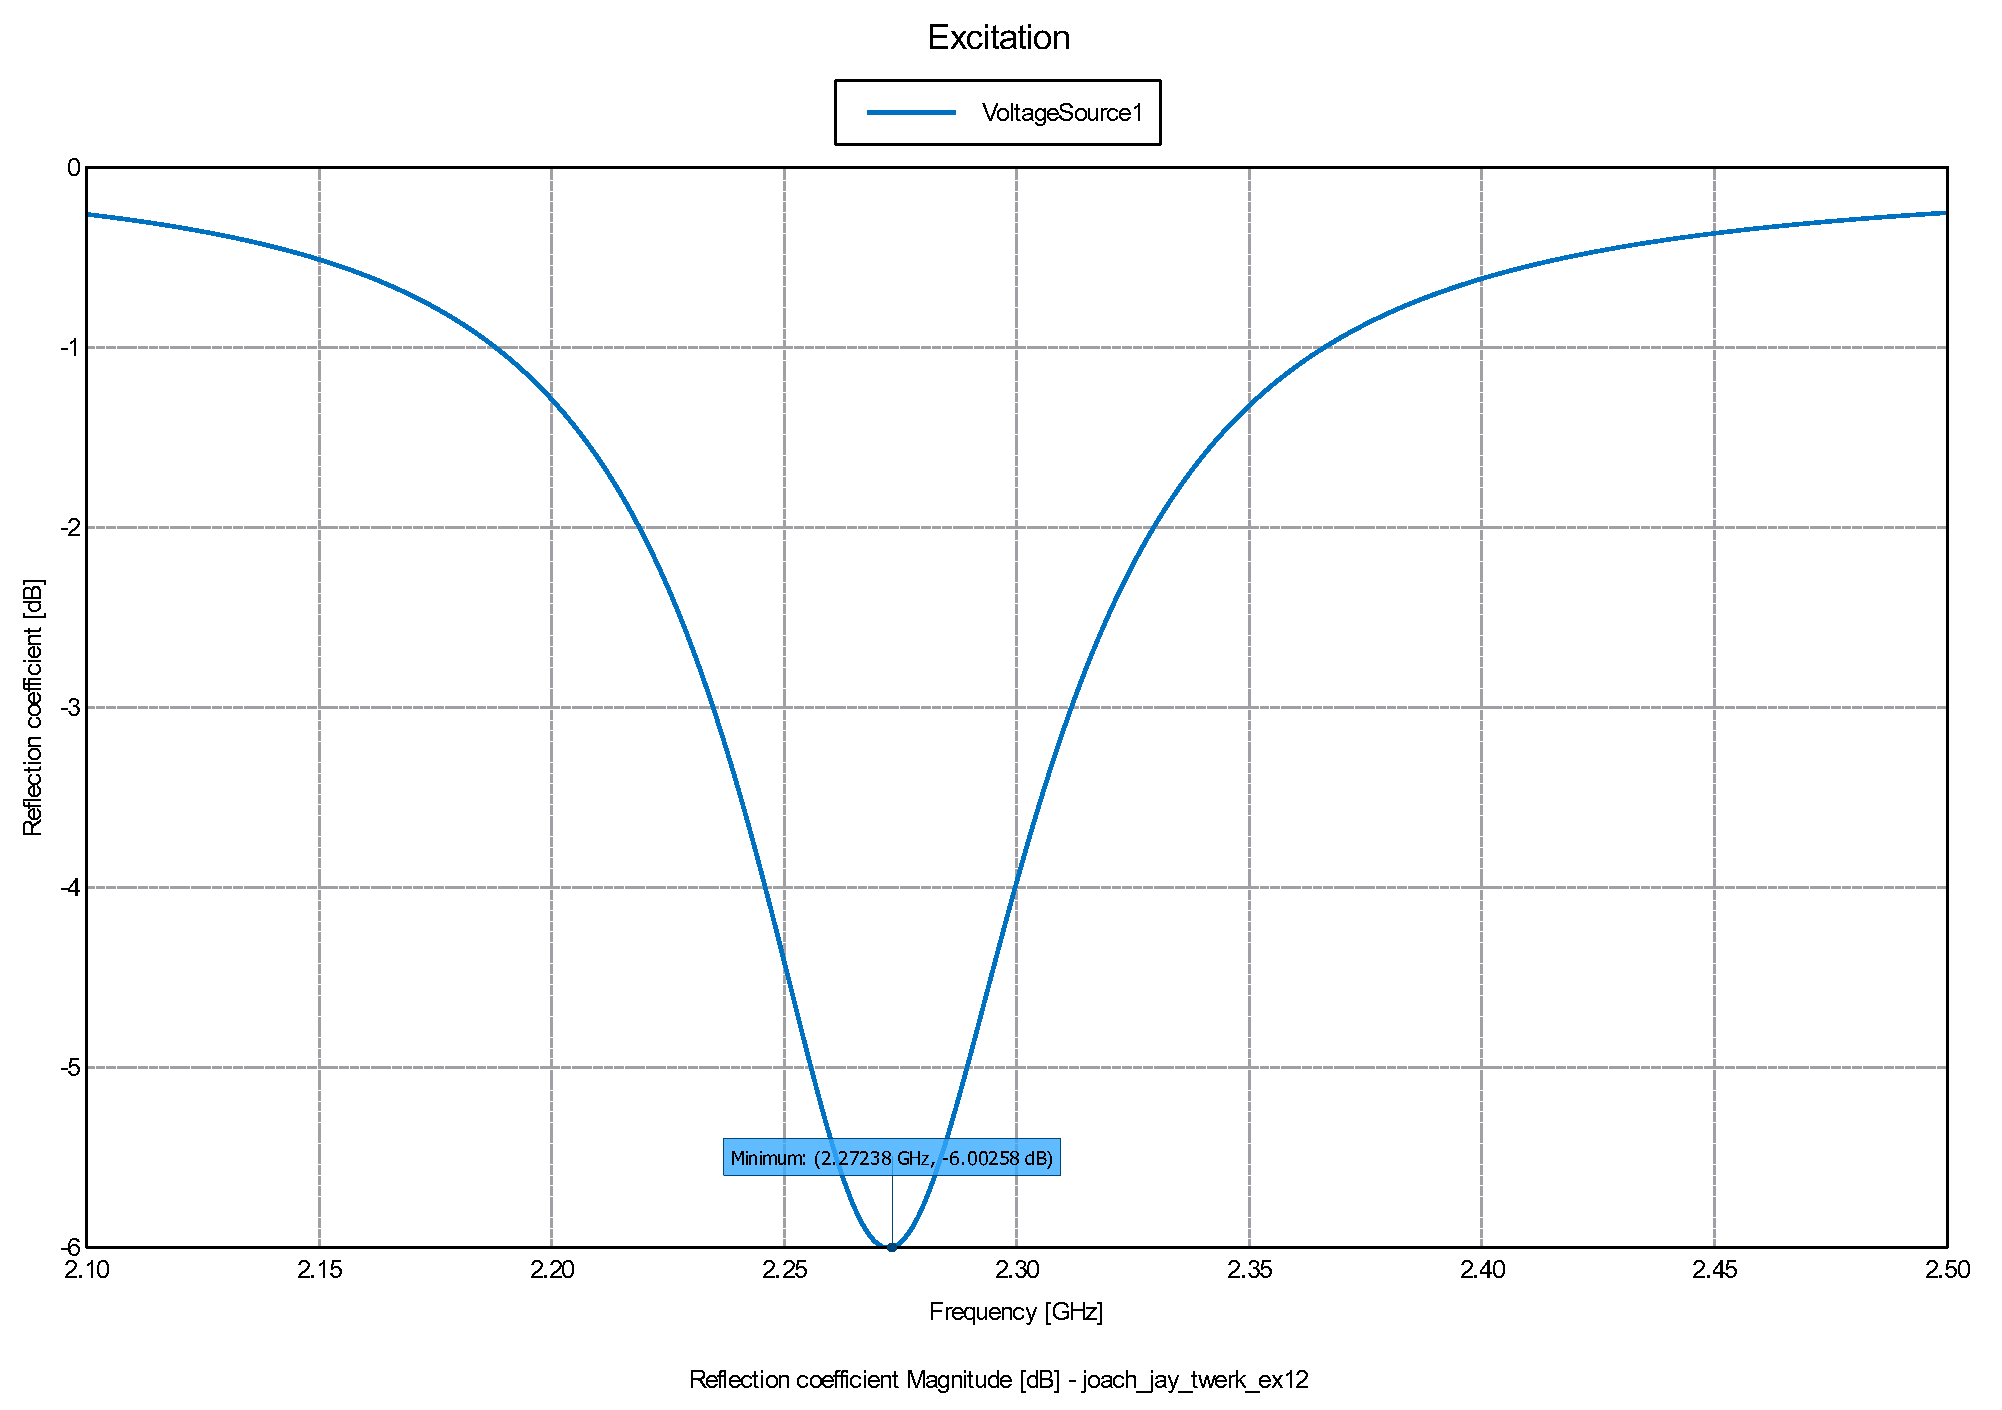
\includegraphics[width=\textwidth]{reflection122_annotation.pdf}
\caption{Coefficient de réflexion en fonction de la fréquence, avec déphasage}
\label{fig:reflection122_annotation}
\end{figure}


\subsection{Antenne avec fente}
Comme l'indique le titre, l'étape suivant a été de "creuser" une fente dans le carré de notre antenne patch. La seule consigne à suivre était que le coefficient de réflexion à la résonance devait être inférieur à \SI{-10}{\deci\bel}. Comme le montre la figure \ref{fig:reflection13_annotation}, notre choix de \SI{8}{\milli\meter} pour $y_0$ respecte cette consigne.
\begin{figure}[htbp]
\centering
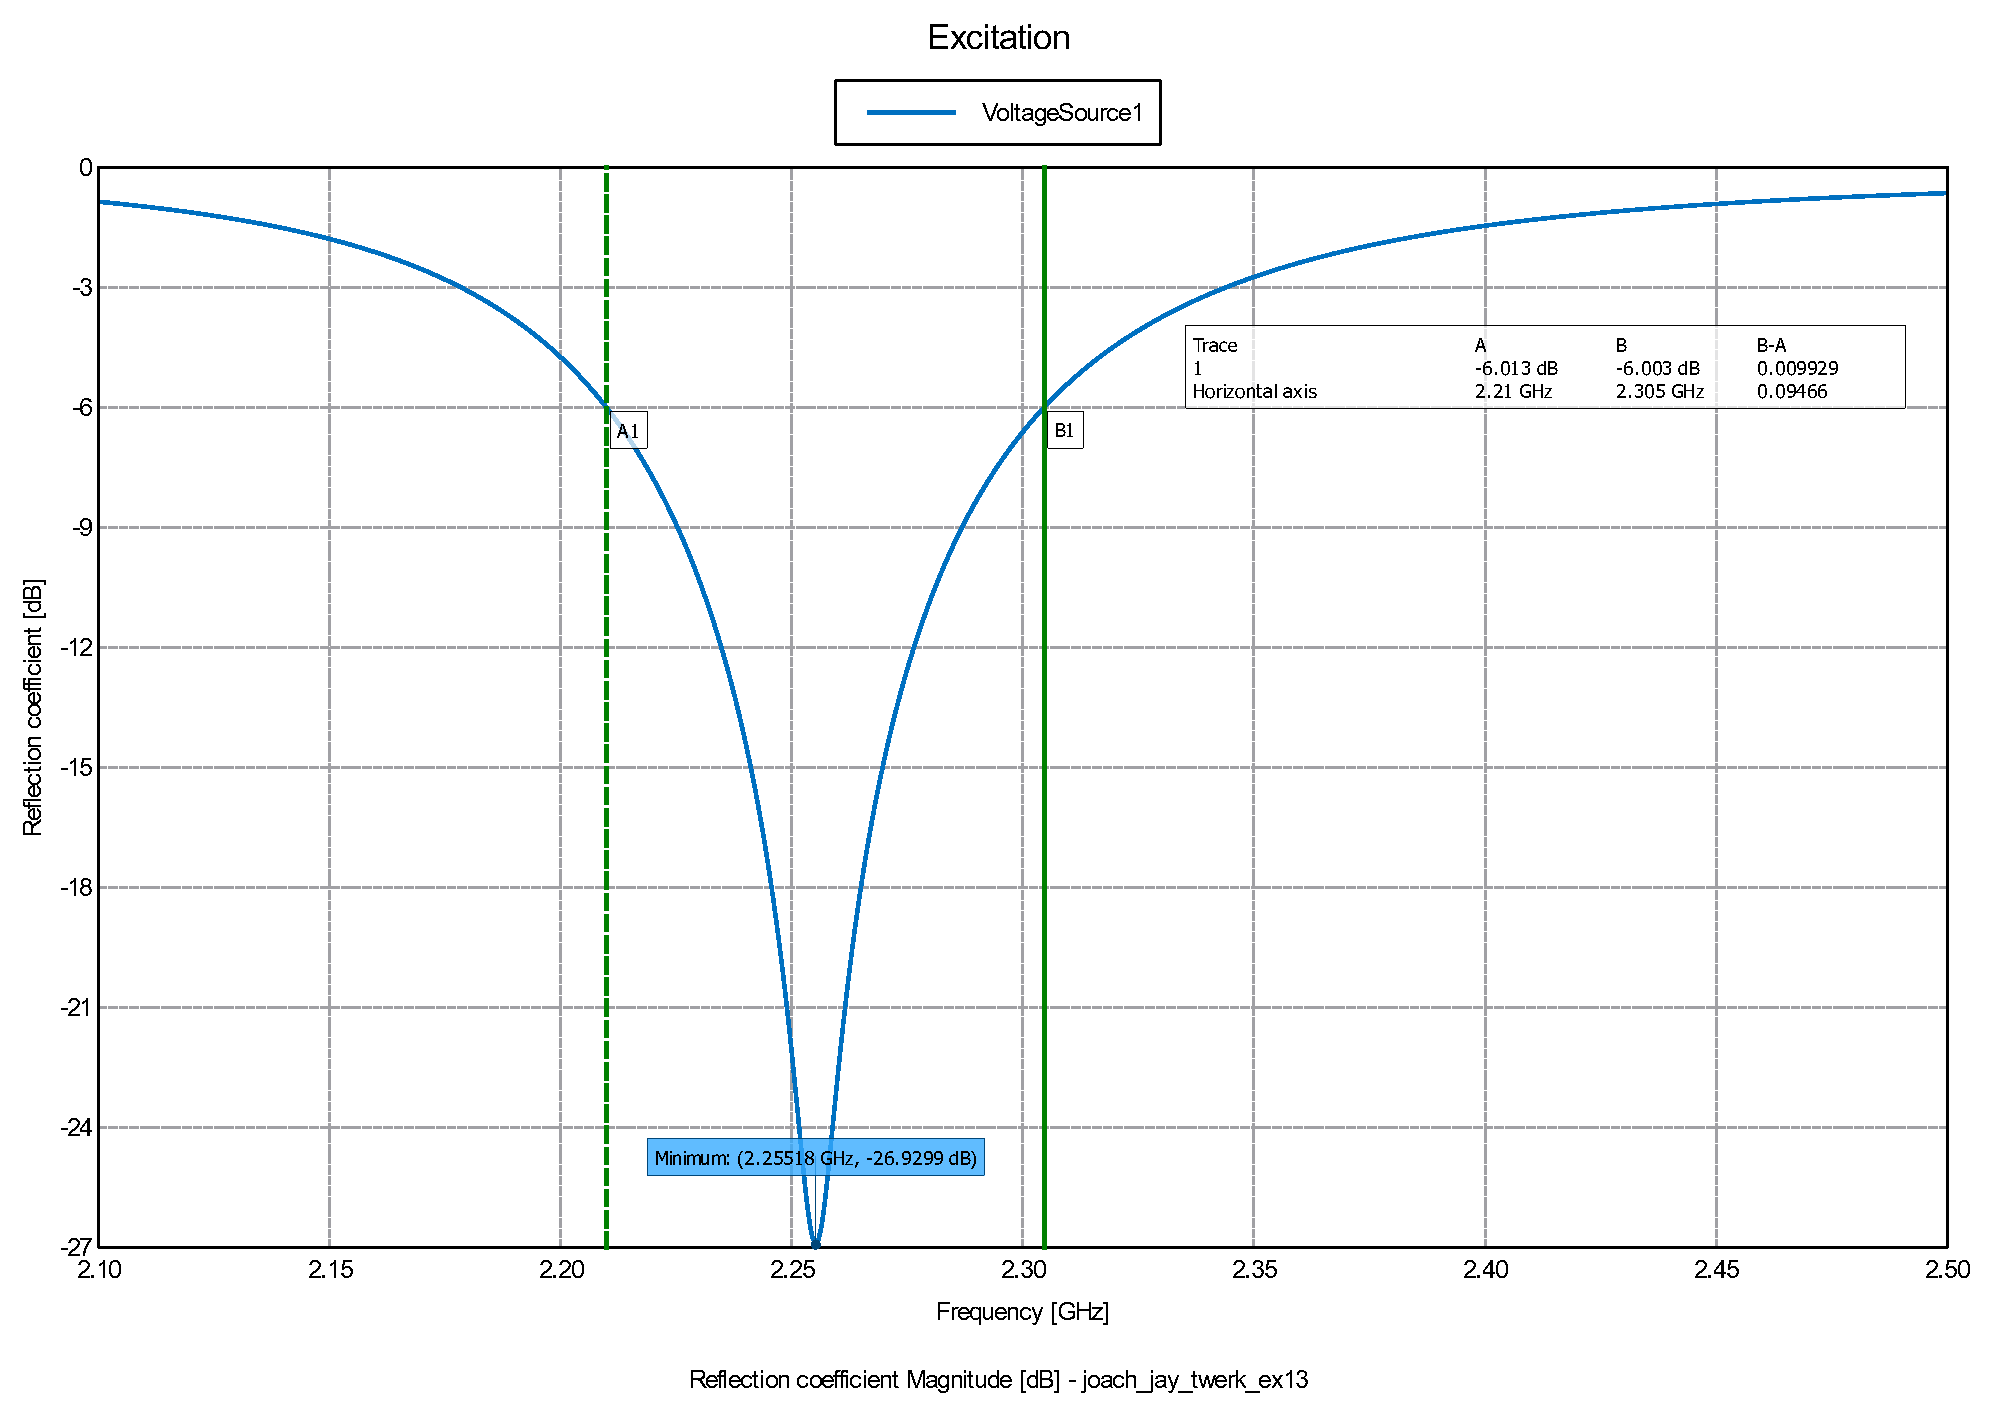
\includegraphics[width=\textwidth]{reflection13_annotation.pdf}
\caption{Coefficient de réflexion en fonction de la fréquence, avec fente de \SI{8}{\milli\meter}}
\label{fig:reflection13_annotation}
\end{figure}

\subsection{Notre antenne}
Pour terminer, nous avons ajouté le microstrip dans la fente de notre patch. Mais ni le coefficient de réflexion, ni la fréquence de résonance ne répondaient au cahier des charges, nous avons donc du modifier les paramètres de notre antenne de manière à s'approcher le plus possible du résultat demandé.
\begin{figure}[htbp]
\centering
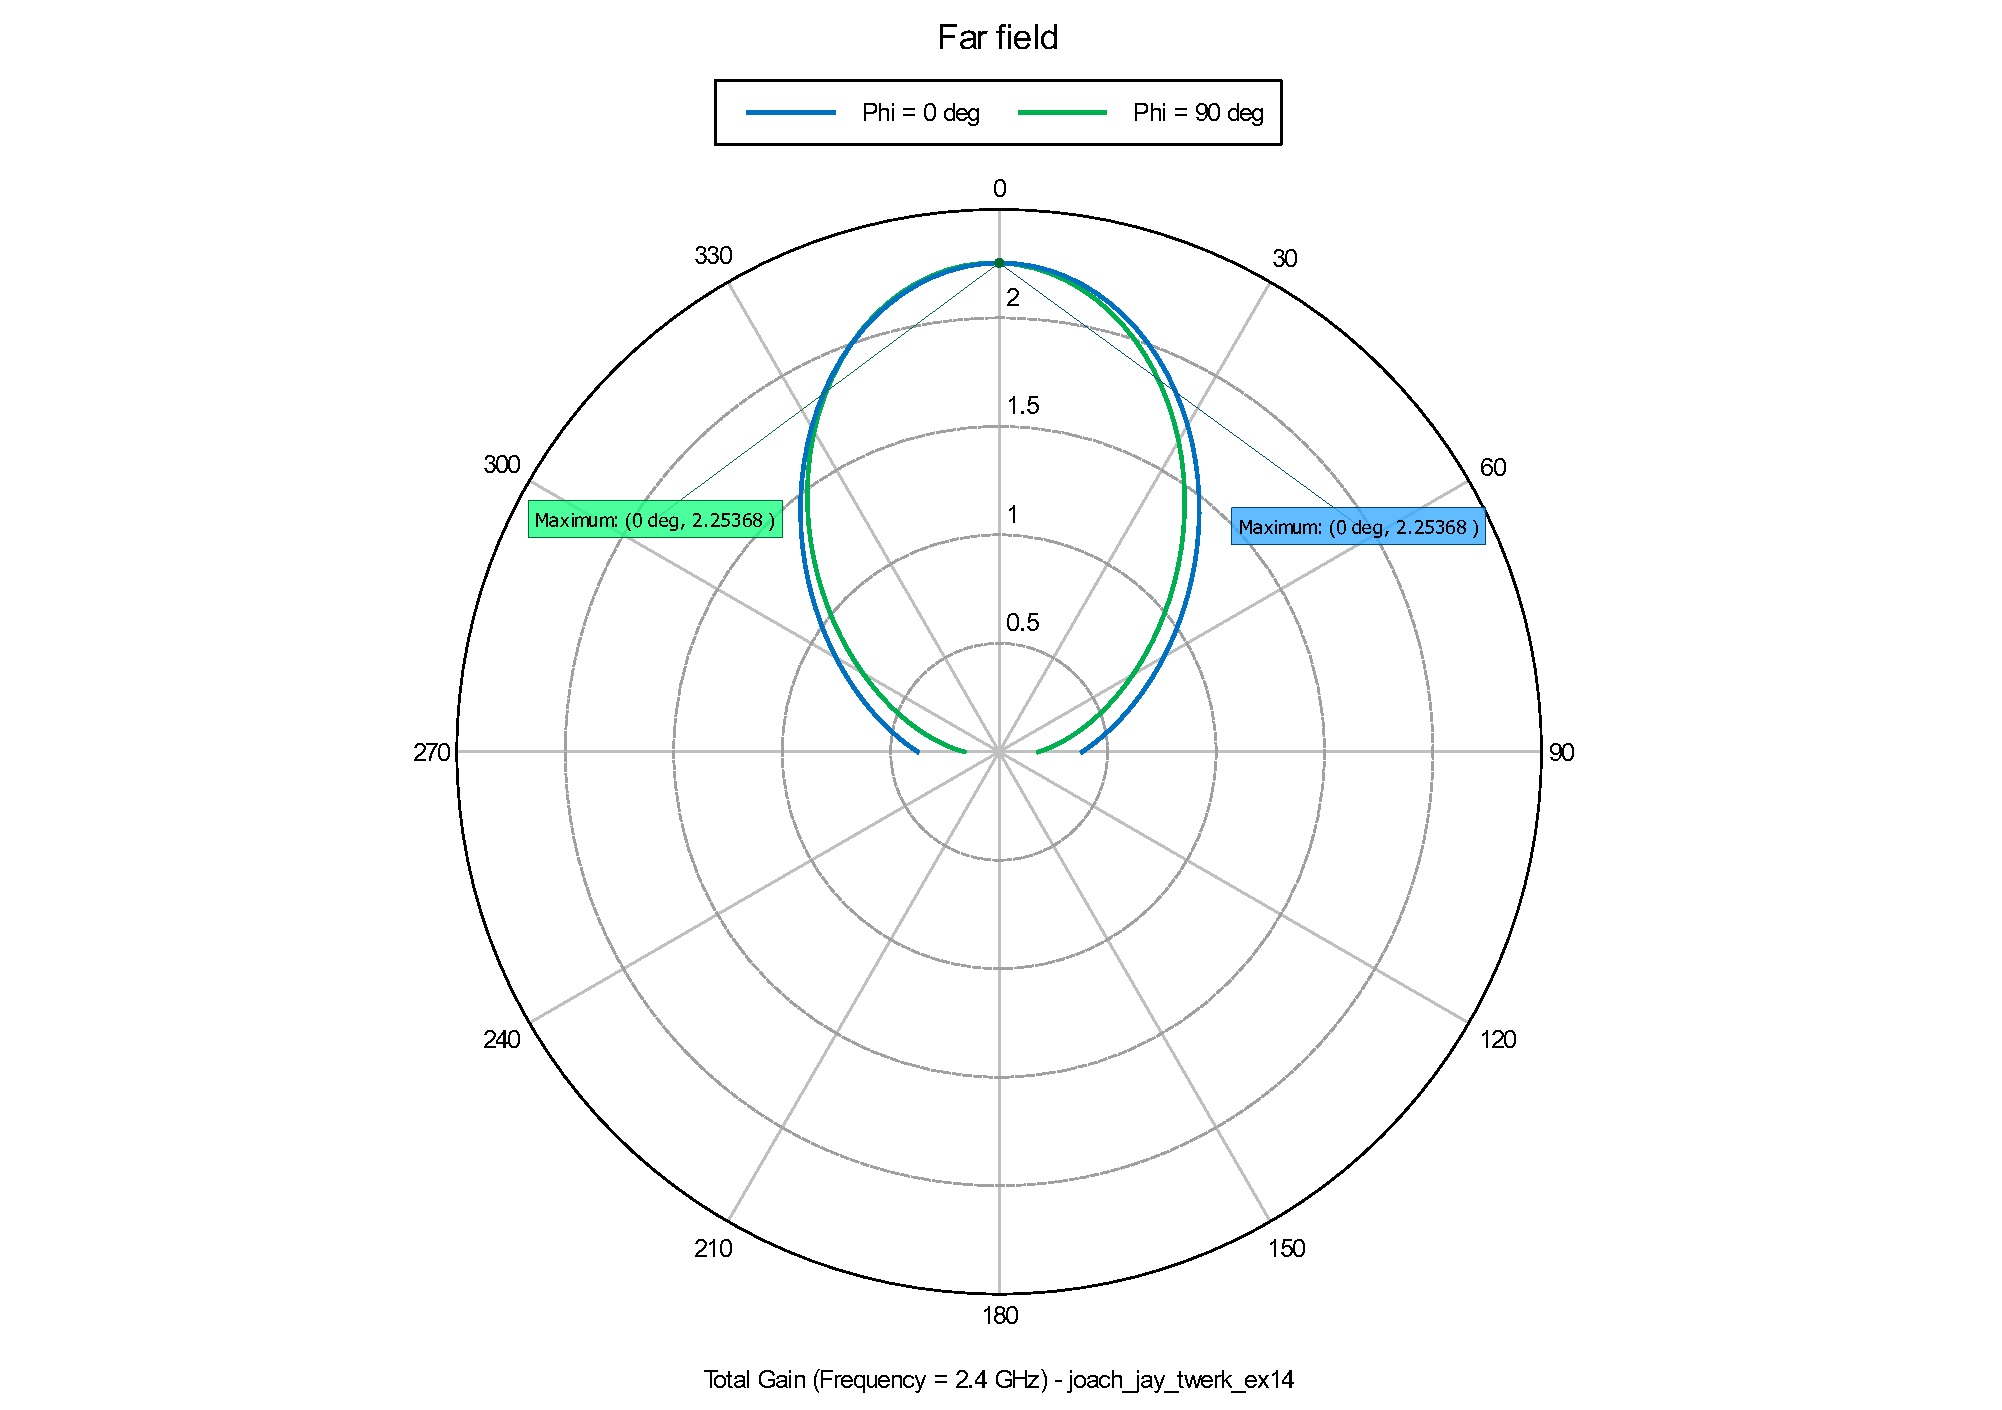
\includegraphics[width=\textwidth]{rayonnement_annotationFinal.pdf}
\caption{Diagramme de rayonnement de notre antenne}
\label{fig:rayonnement_annotationFinal}
\end{figure}
Comme on peut le voir sur la figure \ref{fig:rayonnement_annotationFinal}, notre gain maximum vaut \SI{2.25} pour une directivité de \SI{0}{\degree}. Le coefficient de réflexion est quand à lui donné à la figure \ref{fig:reflection_annotationFinal}.
\begin{figure}[htbp]
\centering
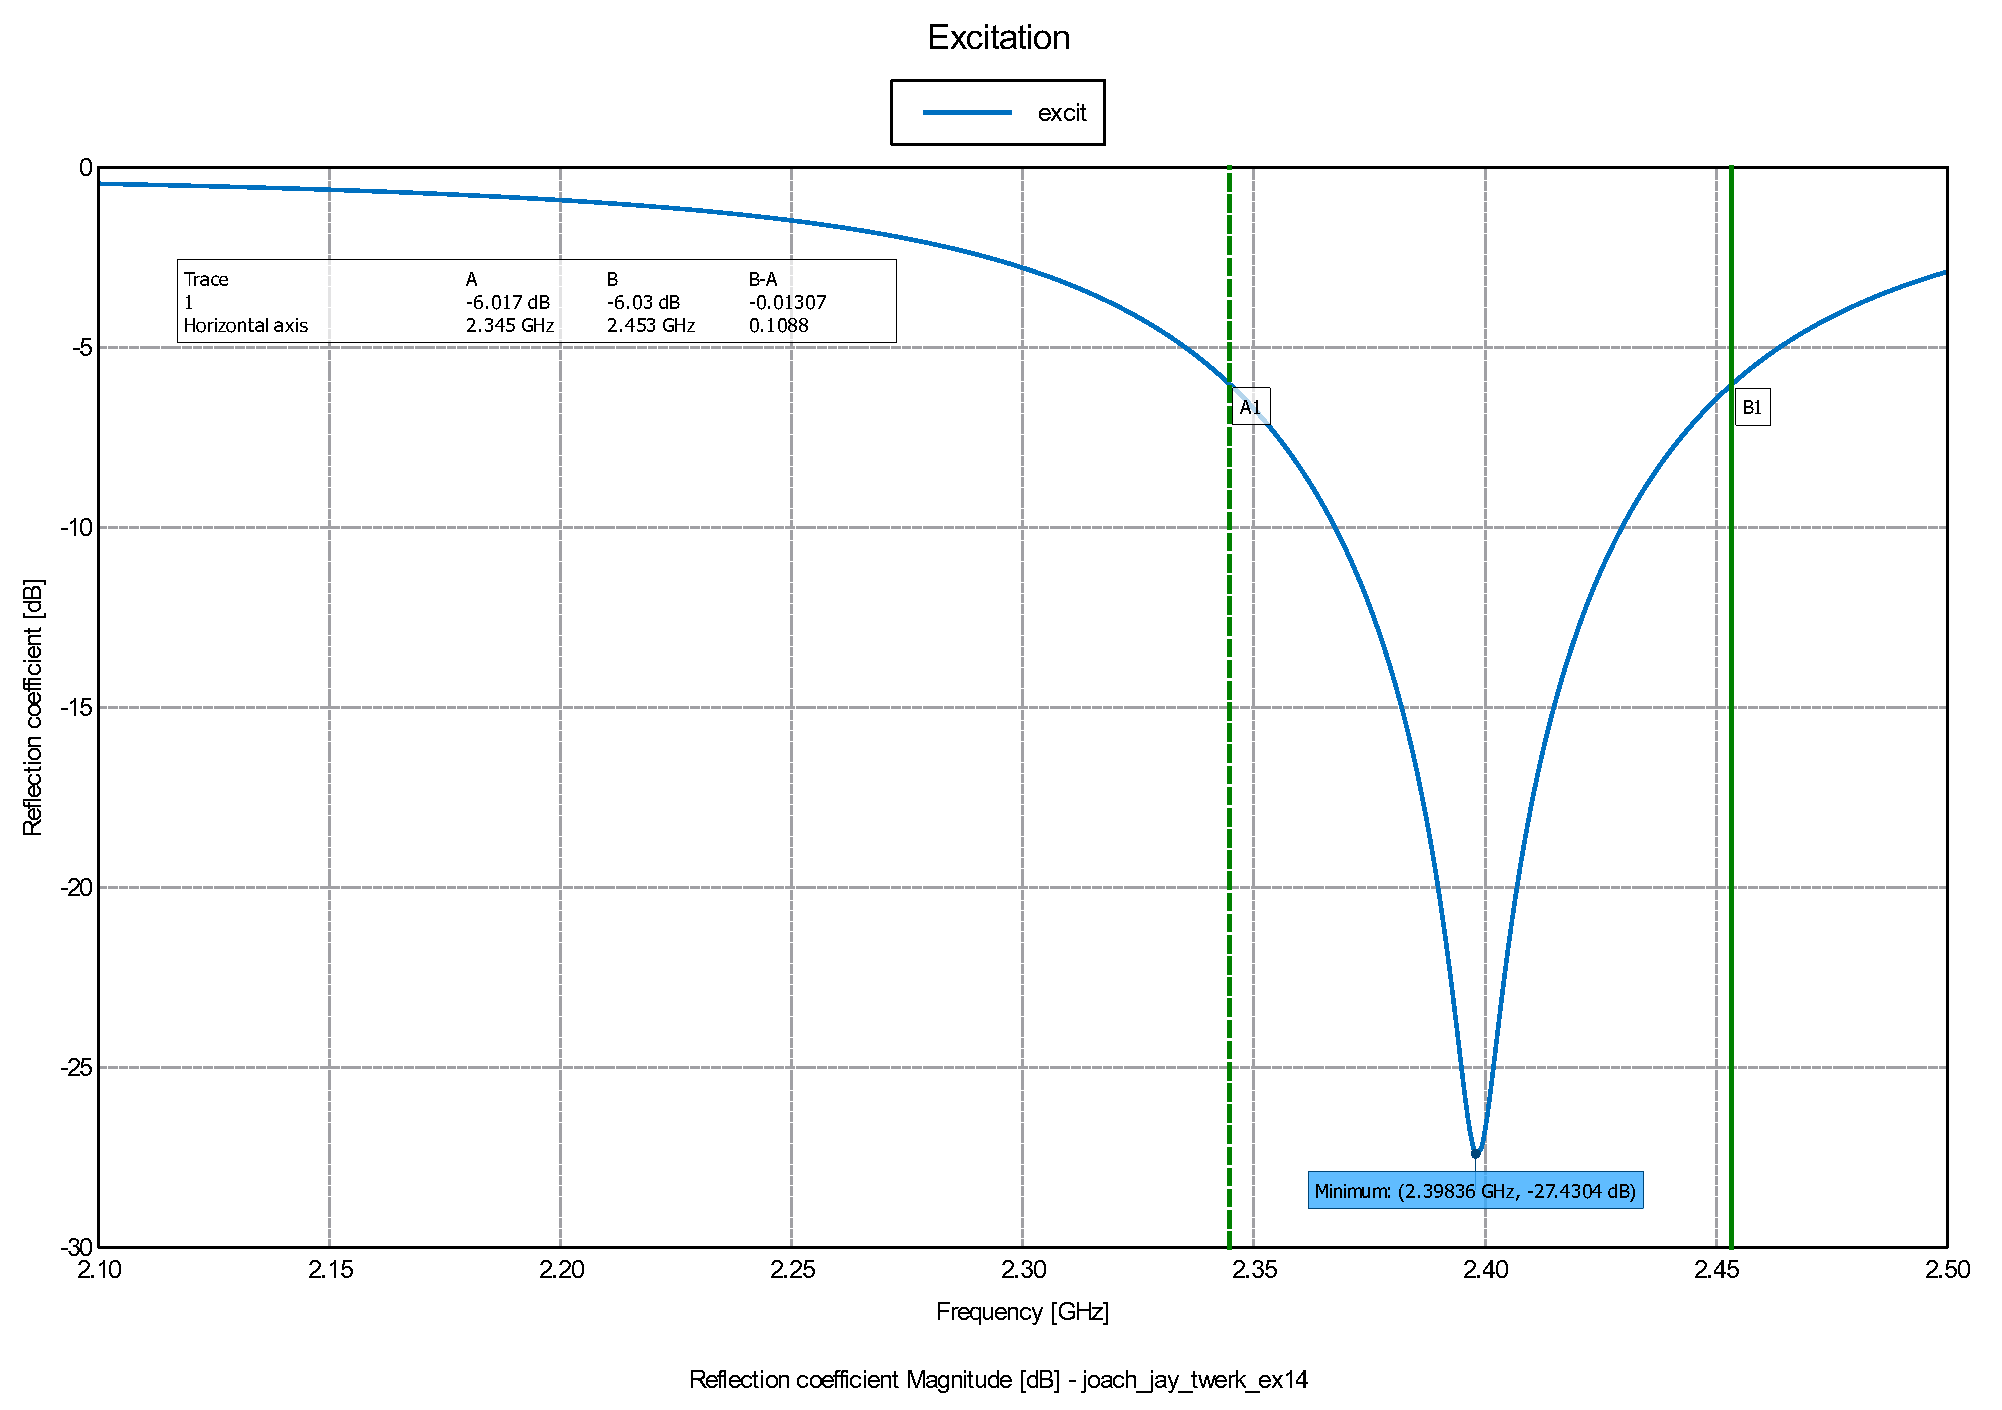
\includegraphics[width=\textwidth]{reflection_annotationFinal.pdf}
\caption{Coefficient de réflexion de notre antenne en fonction de la fréquence}
\label{fig:reflection_annotationFinal}
\end{figure}


%Bonjour, bien dormi?
%Aussi étonnant que ça puisse paraître, \includegraphics[width = x \textwidth]{file.pdf} veut dire que tu redimensionne la figure pour qu'elle soit aussi large que x fois la largeur du texte à cet endroit. A toi d'ajuster à ta guise. Mais ne t'en fais pas, je passerai quand même derrière pour râler malgré tout. U b saf mah nig
